\documentclass{article}

\usepackage{cancel}
\usepackage{amsmath}
\usepackage[includehead,nomarginpar]{geometry}
\usepackage{graphicx}
\usepackage{amsfonts} 
\usepackage{verbatim}
\usepackage{mathrsfs}  
\usepackage{lmodern}
\usepackage{braket}
\usepackage{bookmark}
\usepackage{fancyhdr}
\usepackage{romanbarpagenumber}
%\usepackage{minted}
%\usepackage{subfig}
\usepackage[italian]{babel}
\usepackage{float}
\allowdisplaybreaks

\setlength{\headheight}{12.0pt}
\addtolength{\topmargin}{-12.0pt}
\graphicspath{ {./Immagini/} }

\hypersetup{
    colorlinks=true,
    linkcolor=black,
}

\makeatother

\numberwithin{equation}{subsection}
\newcommand{\tageq}{\tag{\stepcounter{equation}\theequation}}
\AtBeginDocument{%
  \renewcommand{\figurename}{Fig.}
}
\fancypagestyle{link}{\fancyhf{}\renewcommand{\headrulewidth}{0pt}\fancyfoot[C]{Sorgente del file LaTeX disponibile al seguente link: \url{https://github.com/00Darxk/Calcolatori-Elettronici}}}

\begin{document}

\title{%
    \textbf{Calcolatori Elettronici}  \\ 
    \large Appunti delle Lezioni di Calcolatori Elettronici \\
    \textit{Anno Accademico: 2023/24}}
\author{\textit{Giacomo Sturm}}
\date{\textit{Dipartimento di Ingegneria Civile, Informatica e delle Tecnologie Aeronautiche \\
Università degli Studi ``Roma Tre"}}

\maketitle
\thispagestyle{link}

\clearpage


\pagestyle{fancy}
\fancyhead{}\fancyfoot{}
\fancyhead[C]{\textit{Calcolatori Elettronici - Università degli Studi ``Roma Tre"}}
\fancyfoot[C]{\thepage}
\pagenumbering{Roman}

\tableofcontents

\clearpage
\pagenumbering{arabic}


% prof:
% big data
% LLM
% Tirocini (Azienda/Laboratori) 
% Incubare Startup

% scopi del corso
% 6 CFU
% rec 80-85% programma anni precedenti
% cenni di assembly alla fine del corso
% simulatori e casi di studio

%% TODO Introduzione

\section{Storia e Tipologia dei Calcolatori}

%% analisi degli aspetti hardware 
% funzionamento di un microprocessore, facendo riferimento a processori moderni e reali. 

\subsection{Evoluzione delle Architetture}

%% ppt


Un calcolatore è un oggetto che fornisce un risultato, dato un insieme dei dati inseriti. 


L'evoluzione delle architetture dei controllori elettronici si è svolta principalmente negli ultimi settant'anni. Il processo complessivo che ha portato alla nascita 
dei calcolatori moderni viene divisa in generazioni. 
Si chiama generazione zero, l'insieme di calcolatori analogici, progettati per risolvere semplici operazioni, ideati da Pascal e Leibniz. 

Il primo calcolatore programmabile venne ideato da Charles Babbage. Costruì prima una macchina differenziale in grado di calcolare funzioni polinomiali, mentre progettò la 
prima macchina programmabile, completamente analogica, in grado di leggere un input scritto su piastre di rame, e fornire un output, sempre su piastre di rame, utilizzando 
i dati e le operazioni inserite in input. Per poter operare su questi dati di input per fornire istruzioni alla macchina è necessario un linguaggio di programmazione, e la 
prima persona che ha tentato di implementare il linguaggio di Babbage fu Ada. %cognome 


Il passaggio seguente in questa evoluzione venne trainato principalmente dai fondi bellici per realizzare macchine elettromeccaniche. La prima generazione si indica il 
periodo dove vennero realizzati calcolatori abbandonando componenti meccanici. La prima macchina del genere venne create da Alan Turing per decifrare il codice Enigma, 
realizzata tramite valvole, chiamata Colossus. 



Dopo la guerra non servirono più a scopi bellici, per cui si tentò di vendere calcolatori sul mercato, creando la prima società di sviluppo e vendita di calcolatori 
sul mercato, Eniac. 

Negli anni '50 John von Neumann descrisse l'idea di un calcolatore moderno, dove i dati vengono memorizzati su degli indirizzi di memoria. 

L'IBM cominciò la sua storia vendendo calcolatori nel 1953, e continuo ad essere rilevante in questo ambito fino agli anni '80. 
In queste macchine ogni elemento viene definito dal termine ``word'', composto da un certo numero di bit. 


La fine degli anni '50 e l'inizio degli anni '60 vide l'avvento dei transistor, utilizzati in questi anni per la creazione di calcolatori basati su transistor, la società 
rivale della IBM che venne creata in questo periodo fu la DEC. Utilizzando transistor vennero diminuiti i costi, e venne introdotta l'idea di utilizzare uno schermo grafico 
per interagire con l'utente. Il primo calcolatore costruito dalla DEC, PDP-1, fu il primo calcolatore di massa. 

Per accedere ad un calcolatore si utilizzavano dei terminali, tramite un canale di comunicazione chiamato bus, per permettere anche la comunicazione tra elementi interni al 
calcolatore prodotti tra società differenti. 
Si parla comunque di grossi calcolatori per applicazioni scientifiche, militari o di pubblica amministrazione, chiamati ``mainframe'', dove ogni utente accedeva al calcolatore 
tramite terminali. 

Fino agli anni '80 non vennero introdotti cambiamenti radicali all'architettura dei calcolatori, invece i miglioramenti di questi periodi ai calcolatori riguardarono soprattutto 
l'ottimizzazione del software e dell'hardware. 

I primi ``Personal Computer'' vennero introdotti negli anni '80, dall'IBM, che fornì pubblicamente l'architettura del calcolatore. In seguito aumentò in enorme maniera 
l'utilizzo di PC, trainato dall'aumento delle capacità della CPU, e dalla diminuzione dei costi delle memorie principali e secondarie. 


%% ppt... 

% V Computer Invisibili
La maggior parte dei dispositivi moderni contengono microcontrollori, piccoli processori, distribuiti in un contesto completamente pervasivo, su ogni dispositivo collegato 
ad una qualche fonte di energia. Questo concetto viene chiamato anche dell'``Internet of Things''.  

\subsection{Legge di Moore}

Uno dei fondatori dell'Intel, Moore, negli anni '60 definì empiricamente l'omonima legge, secondo cui il numero di transistor su un chip, CPU, memoria, etc., raddoppia ogni 18 
mesi. Questo corrisponde ad un aumento del 60\% all'anno. 

L'evoluzione reale sembra aver seguito l'andamento descritto da Moore, ma recentemente l'evoluzione sta rallentando, a causa dei limiti fisici nella 
realizzazione dei transistor. Per cui esiste un limite superiore al numero di transistor su un unico chip. 
Per misurare la quantità di transistor su un singolo chip si utilizza la grandezza ``Livello di Integrazione'', si riescono a creare chip con un livello di 
integrazione nell'ordine di grandezza dei nanometri, ma livelli di integrazione superiore sono difficilmente realizzabili. Il limite teorico per memorizzare un bit di informazione 
corrisponde allo spin di un elettrone, per cui ci si aspetta una riduzione in questo andamento nei prossimi anni. 

Oltre alla legge di Moore son presenti diverse statistiche per misurare l'evoluzione tecnologica dei processori. Dagli anni 2000 si utilizzano più di un core su un unico 
processo, introducendo semplice forme di parallelismo. Uno dei motivi principali per cui vennero introdotte queste architetture deriva dal limite alla frequenza di funzionamento 
di un processore, poiché all'aumentare della frequenza aumenta il calore prodotto da un processore. Le frequenze maggiori raggiunte da processori si trovano nell'ordine dei 
GHz, queste producono calore fino a 100 Watt. Per aumentare le prestazioni senza aumentare la frequenza, si introducono quindi forme di parallelismo nei processori. Una forma 
semplice consiste nella duplicazione dei componenti, oppure della ``pipeline'', che realizza le stesse prestazioni senza introdurre parallelismo fisico. 
Gia dal 2000 quindi la frequenza operazionale dei processori è rimasta costante, ed ha subito una leggera diminuzione, allo stesso modo del calore generato da un singolo 
processore. Anche se è possibile realizzare processori mono-core che lavorano a frequenze molto elevate, il costo associato al raffreddamento dei componenti non lo rende un 
approccio economicamente attuabile. 

Dal punto di vista tecnologico per migliorare le prestazioni, bisogna cercare forme diverse di realizzazione di processori, che non utilizzano transistor, una di queste possibili 
tecnologie riguardano la computazione quantistica. 


La legge di Nathan afferma che il software è un gas, riempie sempre completamente qualsiasi contenitore in cui viene inserito. Per cui molto velocemente e facilmente un 
calcolatore diventa obsoleto, questo alimenta un circolo vizioso che spinge l'evoluzione tecnologica, e rappresenta quindi la legge di Moore. 

\subsection{Tipologie di Processori}

Un calcolatore è un dispositivo in grado di ricevere dei dati, di memorizzare in piccola parte i dati, di elaborare i dati, e di produrre un output. In generale un qualsiasi d
dispositivo elettronico in grado di soddisfare queste quattro specifiche può essere considerato un calcolatore. 
Si possono quindi definire diverse classi di calcolatori o processori sulla base delle loro prestazioni, all'aumentare delle prestazioni aumenta quindi il costo associato ad 
un dato processore. Esistono calcolatori monouso o ``usa e getta'', e microprocessori di basso costo, utilizzati negli elettrodomestici, automobili, o altri oggetti che non richiedono di capacità 
di computazione elevate, e soddisfano compiti specifici. Processori più evoluti, ma sempre specializzati, vengono utilizzai per applicazioni ``mobile'', oppure per piattaforme 
di gioco. L'unica differenza rispetto ad un Personal Computer è la loro specializzazione, mentre i processori di questa categoria svolgono applicazioni più generali 
``General Purpose'', in grado di essere programmati. Processori ancora più avanzati vengono utilizzati per fornire servizi, non per l'elaborazione personale, e vengono chiamati 
server, ma in termini di tecnologia non presenta differenze evidenti rispetto ad un PC. Veniva utilizzati processori ancora più potenti, chiamati ``Mainframe'', sulla base della 
centralizzazione della computazione, dove un singolo processore soddisfa le richieste di tutti gli utenti, ma non vengono più utilizzati a favore dell'elaborazione 
distribuita. 


Processori usa e getta come gli RFID ``Radio Frequency IDentification'' rappresentano la categoria di processori più diffusa, sono tipicamente passivi, senza batteria, ma esistono 
dispositivi attivi, di dimensione 
molto contenuta, nell'ordine di qualche millimetro, contenente un piccolo processore dotati di un transponder radio. Contiene una memoria di 128 bit complessivi. Il transponder 
è in grado di ricevere segnali su una certa frequenza, inviato da un lettore, questo segnale radio fornisce ulteriormente l'energia necessaria per alimentare il processore 
che invia il numero memorizzato in memoria. 
Gli RFID attivi dotati di una batteria non necessitano di essere molto vicini al lettore per operare, uno di questi dispositivi è il ``Telepass''. 


Microprocessori sono oggetti di plastica che contengono un processore, una piccola memoria, e forniscono un collegamento con l'esterno da vari piedini metallici. Necessitano di 
un'alimentazione esterna, su uno di questi piedini. Questi processori non sono programmabili, e vengono usati in applicazioni di controllo. 


Processori specializzati, non estendibili, ma di prestazioni molto superiori ai microprocessori sono i ``Game Computer'', che presentano effetti grafici speciali, per cui 
in generale presentano un processore grafico specializzato ``Graphical Processing Unit'' o GPU, ed un software di base limitato. Oltre alla memoria di base chiamata RAM, contengono la memoria di video, per gestire 
la visualizzazione a schermo chiamata VRAM. Generalmente questi processori CPU o GPU lavorano a non più di 4 GHz, per fornire informazioni sulle prestazioni di un processore 
si considera la banda di un processore, che rappresenta il numero di operazioni effettuabili in un dato intervallo di tempo. Si usa l'unità di misura FLOPS ``FLOating points Per Second'' 
supponendo il caso peggiore, quindi operazioni su numeri a virgola mobile. In generale questi dispositivi presentano una banda nell'ordine dei tera FLOPS. 
Questi sistemi sono chiusi, quindi non è possibile aumentare le prestazioni aggiungendo ulteriori chip al dispositivo. 
Appartengono alla stessa categoria le applicazioni Mobile, che presentano processori anche a otto core, con frequenze inferiori, poiché non presentano un sistema di raffreddamento 
attivo, e contengono una batteria e non un'alimentazione costante, per cui si utilizzano queste frequenze per diminuire il consumo energetico del processore. I processori 
utilizzati nell'ambito Mobile appartengono alla famiglia ARM, questa non è una casa produttrice come Intel o AMD, ma rappresentano una categoria di processori che vengono 
realizzati da diversi produttori, poiché è un'architettura aperta, di cui sono note le specifiche ed il linguaggio macchina. Questo modello di mercato si basa interamente sulle 
licenze vendute dalla casa produttrice ARM, per cui si quando si parla di un processore di questa famiglia, si include anche la casa produttrice che ha prodotto il processore. 
Recentemente la Apple ha esteso l'uso di processori ARM anche su applicazioni di Personal Computer. Su questi dispositivi le funzionalità I/O vengono fornite tramite un 
'interfaccia grafica basate su touch-screen. 


Il Personal Computer si riferisce alla disciplina dell'elaborazione personale dei dati. Sono processori di specifiche non molto diverse dalle precedenti, ma sono 
programmabili. Tutti questi dispositivi sono connessi alla rete, per cui appartengono all'Internet of Things. La differenza tra un PC ed un server è la disciplina secondo cui 
l'elaborazione dei dati non è personale, ma fornisce un servizio. Tipicamente questi servizi vengono fornite tramite diversi server che lavorano in parallelo secondo la 
disciplina COW ``Cluster Of Workstation'', collegati 
tramite una rete ad alta velocità, che presentano una ridondanza nella replicazione dei dati, in caso uno di questi server abbia un malfunzionamento. La tendenza al parallelismo 
è quindi presente non solo a livello microscopico sui singolo processori, ma anche a livello macroscopico utilizzando più server. Permettono di continuare ad erogare il servizio in 
caso di un malfunzionamento, ed è molto raro che la maggior parte dei server nel cluster falliscono contemporaneamente. La realizzazione di questi server segue la disciplina 
della scalabilità orizzontale, ovvero vengono aggiunti nuovi server all'aumentare degli utenti, quando invece è presente un unico server si parla di scalabilità verticale, dove 
per fornire servizi a più utenti si aumentano le prestazioni di un unico server. 


Esiste una tendenza di molte organizzazione a non realizzare un sistema di elaborazione con risorse proprie, ma utilizzare risorse nel Cloud, un'esempio molto diffuso è l'AWS, 
o gli Amazon Web Service, che forniscono memoria, memorizzazione di dati, e capacità di computazione accessibile nel Cloud. In questo approccio si sta ritornando all'approccio 
del Mainframe, ma in questo caso il terminale di accesso alle risorse fornite nel Cloud è anch'esso un calcolatore avente risorse di calcolo proprie, per elaborare una 
parte dei dati ``In Premise''. 



Verranno trattati tre diversi tipi di processori, appartenenti alla famiglia Intel e ARM, ed un processore appartenente alla famiglia dei microcontrollori della famiglia AVR.
\subsubsection{Architettura Intel}
%% ppt

Il primo processore commercializzato dalla Intel è il 4004, con una frequenze tra le frazioni di un MHz, ed in grado di gestire poche centinaia di bit di memoria. Una variante 
di questo processore, specializzato per microcontrollori il 8008, fornì la base per la creazione del primo processore ``general purpose'' su un circuito integrato, il 8080.  

La prima cifra nel nome corrisponde al tipo di architettura del processore, indica il numero di bit in cui vengono salvati e gestiti i dati sui registri del processore. 
A partire dagli anni '90 si cominciò ad utilizzare nomi diversi dai numeri per indicare i processori. Si introdussero memorie cache, ed all'inizio degli anni 2000 si introdussero 
diverse forme di parallelismo fisico, e non solo, mantenendo le frequenze inferiori ai 4 GHz. Per molti anni si utilizzava lo stesso processore anche per la gestione 
dello schermo, ma già da parecchi anni è la norma utilizzare due processori separati. 
%% core i3, i5, i7, i9, xeon
Tutti i processori moderni della stessa famiglia sono compatibili con lo stesso linguaggio macchina. La denominazione di un processore indica le sue prestazioni, e sono 
quindi destinati a diversi settori di mercato, per cui l'evoluzione non dipende più dal nome del processore, ma dalla generazione dei processori. Attualmente ci si trova 
in una generazione intermedia tra la tredicesima e la quattordicesima, in generale un salto generazionale viene definito dal livello di integrazione, i processori moderni 
hanno un livello di integrazione di 7 nanometri. 
Sono tutte architetture che presentano fino ad otto core, ma recentemente invece di utilizzare core identici sullo stesso processore sono state introdotte architetture ibride 
i cui core sono di almeno due forme diverse chiamati ``p-core'', per le prestazioni in termini di calcoli complessi, e gli ``e-core'', sono più efficienti in termini di consumo 
di energia. POssono avere fino a 24 stadi di pipeline, che permettono di avere altre forme di parallelismo, senza utilizzare parallelismi fisici. 

Utilizzando un'unica catena di produzione, in base alla qualità in cui vengono prodotti si ottengono diversi processori, disattivando le componenti che non funzionano 
correttamente sul processore, e si vendono quindi come dei processori aventi prestazioni minori rispetto ad una versione completamente funzionante. 

Il processore Intel Core i7 presenta sei core abilitati su otto core disponibili, la sua versione completamente abilitata corrisponde al processore Xeon. Presenta poco più di 
un miliardo di transistor ed un livello di integrazione nell'ordine dei 22 nanometri. 

%% ppt. 

\subsubsection{Architetture ARM}

La società Acorn inventò negli anni '80 questo tipo di architettura bastata sui principi RISC (Acorn RISC Machine). Venne usato sui primi tablet prodotti dalla Apple. Nasce come 
un processore integrato ed a basso consumo energetico. Presenta un modello di commercializzazione diverso rispetto al resto del mercato, utilizzano un'architettura aperta, che 
permette a diverse case produttrici di realizzare questi processori, vendendo le licenze per poter produrre il processore. Ogni processore ARM viene quindi accompagnato dal nome 
dell'azienda che l'ha realizzato. 

Si analizzerà in seguito l'Nvidia Tegra 2, un SOC ``System Of a Chip'' contenente due processori della famiglia ARM, una piccola GPU ed ulteriori componenti.  

\subsubsection{Architettura AVR}
L'architettura AVR corrisponde a processori progettati per elettro-domestici, e per funzioni specifiche. Nacque da un progetto universitario del NIT nel 1996, dal nome dei 
suoi creatori Alf and Vergard RISC Processor. Presenta lo stesso pinout dell'8051 Intel. Presenta vari timer, un orologio interno, trasmettitore di impulso, interfaccia 
di sensori, convertitori analogico-digitali, transponder e comparatore di tensioni. Presenta memorie nell'ordine delle centinaia dei kilobyte per la memoria persistente Flash, 
una memoria programmabile da poche migliaia di byte ``EEPROM'', ed una memoria principale fino ad un massimo di 16 KB, per i microcontrollori più potenti. 

\clearpage

\section{Sistemi di Numerazione Binaria}

%% TODO unità di misura (ppt.) 

Quando si misura la memoria si utilizza l'unità di misura byte, corrispondente a 8 bit, e si tende ad utilizzare potenze di due invece di potenze di dieci, utilizzando 
i bit quando si considera una velocità. 

Si utilizza questa notazione per la struttura fisica della memoria, la cua dimensione viene definita dal numero di bit di un indirizzo binario. Dato un indirizzo definito da 
$n$ bit, sono possibili $2^n$ indirizzi distinti di memoria. Per cui è più semplice lavorare con potenze di due quando si analizza la memoria. 

Nei sistemi di numerazione binaria è presente una differenza sostanziale tra il concetto di numero, un entità astratta, ed il concetto di numerale, 
una sua possibile rappresentazione in un dato sistema di numerazione. 
Nell'ambito dei calcolatori elettronici il numero di caratteri diversi per poter rappresentare un numero è finito, poiché lo è la dimensione dei registri di memoria. Per cui 
i numeri possono essere rappresentati a precisione finita, e si perdono alcune proprietà come la chiusura rispetto alle sue operazioni, sono presenti errori di arrotondamento di 
un numero, ciò corrisponde ad un errore di ``overflow''. Inoltre non è possibile rappresentare tutti i numeri reali, essendo infiniti, per cui possono essere rappresentati solo 
numeri con un numero finito di cifre decimali in un dato intervallo. 

\subsection{Rappresentazione a Virgola Fissa}

In generale un numero viene rappresentato rispetto ad una base $b$, dove ciascuna cifra $a_i$ del numerale rappresenta il coefficiente di una potenza della base $b$:
\begin{gather*}
    N:a_m\cdots a_0,a_{-1}\cdots a_{-k}\\
    N=\displaystyle\sum_{i=-k}^ma_ib^i
\end{gather*}
Questa rappresentazione viene chiamata posizionale. 
Per rappresentare un numero utilizzando una base $b$, sono necessari $b$ simboli distinti per poter rappresentare tutte i possibili coefficienti. Dopo aver 
esaurito le dieci cifre arabe $0,\cdots,9$ bisogna utilizzare diversi caratteri, per basi esadecimali si usano lettere dell'alfabeto per completare l'alfabeto di simboli 
utilizzato $A,\cdots,F$. 
Ogni numerale deve essere quindi associato alla sua base per poter ricavare le informazioni del numero che rappresenta.  

Questa rappresentazione si dice a virgola fissa, poiché viene definito a priori tramite il parametro $k$ il numero di cifre dopo la virgola utilizzate. 

\subsubsection{Sistema Posizionale}
Per rappresentare l'insieme dei numeri naturali, viene utilizzata il sistema posizionale, in notazione binaria con $n$ bit si possono esprimere tutti i numeri nell'intervallo 
$[0,2^n-1]$. Si sfruttano quindi tutte le $2^n$ posizioni disponibili, dove devono essere rappresentati per ogni numerale anche gli $0$ non significativi.  

Le operazioni aritmetiche di base come la somma si svolgono cifra a cifra, portando il resto sulla cifra successiva, in caso il risultato non possa essere rappresentato 
utilizzando $n$ bit si ha un errore di overflow, o trabocco, nella propagazione del resto. 
Anche la moltiplicazione viene effettuata cifra a cifra tra i due numerali, poiché sono presenti solo due simboli in base due, i prodotti parziali sono pari a zero, oppure 
al moltiplicando, la somma tra i prodotti parziali si svolge come descritto precedentemente. Inoltre è possibile si verifichi un errore di overflow sulle moltiplicazioni, 
molto più facilmente rispetto ad una somma. 

Il sistema posizionale include la rappresentazione di numeri con una parte decimale, può essere rappresentato utilizzando $n$ bit, fissata la posizione della virgola nel 
numerale. Si possono così rappresentare numeri a parte decimale positivi. In questo modo è possibile effettuare le operazioni di somma allo stesso modo dei numeri naturali. 
Nella moltiplicazione non si possono rappresentare ulteriori cifre decimali, per cui si perde precisione effettuando questa operazione tra due numerali a virgola fissa. 
Moltiplicare un numerale per $2^n$ corrisponde a spostare la virgola di $n$ posizioni a sinistra, mentre per $2^{-n}$ corrisponde a spostare la virgola di $n$ posizioni a 
sinistra. 

\subsubsection{Rappresentazione tramite Modulo e Segno}
Per rappresentare i numeri con segni è necessario modificare il sistema posizionale, sono possibili diverse variazioni per ottenere questo risultato. 
Una di queste si indica 
come rappresentazione per modulo e segno, dove il primo bit del numerale indica il segno del numero, se è $0$ è positivo, mentre se è $-1$ è negativo, mentre si usano $n-1$ bit 
per il modulo. In questo modo si riduce l'intervallo di rappresentazione, potendo rappresentare numeri su un intervallo simmetrico $[-2^{n-1}+1,2^{n-1}-1]$, ma sono 
possibili due rappresentazioni per lo zero $\pm0$

\subsubsection{Rappresentazione Complemento ad Uno ed a Due}
La rappresentazione complemento a 1 si aggiunge uno zero a sinistra, si utilizza la rappresentazione posizionale per numeri positivi, mentre per numeri negativi si rappresenta 
il modulo nella rappresentazione posizionale, ed in seguito si complementa il numerale bit a bit. L'intervallo di rappresentazione coincide per la rappresentazione per modulo e segno 
$[-2^{n-1}+1,2^{n-1}-1]$, ed allo stesso modo è presente una doppia rappresentazione dello zero. 


Per evitare la doppia rappresentazione dello zero si utilizza il sistema della complementazione a due, una piccola variante del complemento ad uno. Se il numero è positivo si 
utilizza la rappresentazione posizionale, mentre per un numero negativo si rappresenta il suo modulo con la rappresentazione posizionale, si complementa bit per bit e si somma ad 
uno. In questo modo l'intervallo di rappresentazione con $n$ bit coincide a $[-2^{n-1},2^{n-1}-1]$, ed è possibile un'unica rappresentazione dello zero. Per cambiare di segno 
di un numerale in questa rappresentazione è sufficiente complementare a due il numerale. 
%% TODO ppt. somma cp2  
Nel sistema a complemento a due per effettuare l'operazione di somma è sufficiente svolgere una somma bit a bit, si verifica un overflow se la somma tra due numerali dello 
stesso segno cambia il segno, altrimenti bisogna ignorare il trabocco ed il risultato è sempre corretto. Per svolgere l'operazione di differenza si cambia di segno il secondo numerale e si svolge una somma.  
Le moltiplicazioni tra due numerali in questa rappresentazione si svolgono tra i valori assoluti, e se necessario si complementa il risultato. 

\subsubsection{Rappresentazione ad Eccesso}
Esiste un'altra rappresentazione chiamata ad eccesso. Dati $n$ bit, si definisce un numero noto chiamato eccesso, generalmente $2^{n-1}$. Può rappresentare numeri sullo stesso 
intervallo della rappresentazione a complemento a due. Per rappresentare un numero si somma all'eccesso, ottenendo un numero sicuramente positivo per cui si può rappresentare 
utilizzando semplicemente il sistema posizionale. In pratica i numerali si ottengono da quelli della rappresentazione a complemento a due, complementando il bit più significativo. 
In questa rappresentazione i numerali sono disposti sequenzialmente dal più piccolo al più grande, a distanza di uno tra di loro.  


Si considerano le rappresentazioni trattate precedentemente a confronto tra di loro, con 3 bit: 
\begin{center}
    \begin{tabular}{|c||c|c|c|c|}
        \hline
        Decimale & Modulo e Segno & Complemento a 1 & Complemento a 2 & Eccesso a 4\\
        \hline\hline
        +3 & 011 & 011 & 011 & 111 \\
        \hline
        +2 & 010 & 010 & 010 & 110 \\
        \hline
        +1 & 001 & 001 & 001 & 101 \\
        \hline
        +0 & 000 & 000 & 000 & 100 \\
        \hline
        -0 & 100 & 111 & & \\
        \hline
        -1 & 101 & 110 & 111 & 011 \\
        \hline 
        -2 & 110 & 101 & 110 & 010 \\
        \hline
        -3 & 111 & 100 & 101 & 001 \\
        \hline
        -4 & & & 100 & 000 \\
        \hline
    \end{tabular}
\end{center}
I bit più significativi si trovano sempre verso destra, e rappresentano l'ordine di grandezza del numero. In tutti questi sistemi, 
il primo bit, il più significativo, identifica sempre il segno del numerale e dipende dalla rappresentazione usata. 


Un numerale identifica solamente una sequenza di cifre, il numero corrispondente dipende dalla rappresentazione, e questa deve essere necessariamente fornita, insieme al numerale, per poter associato ad un numero. 

\subsection{Rappresentazione a Virgola Mobile}

La rappresentazione di numeri tramite virgola fissa non è un sistema efficiente, poiché si usa lo stesso numero di bit, per tutti i numeri di ordini di grandezza diversi, quindi spesso le cifre più significative 
non forniscono informazioni aggiuntive per poter identificare il numero, e sono quindi superflue. Per poter ovviare a questo problema si considera una rappresentazione detta a virgola mobile, o ``floating point'', 
dove l'ordine di grandezza è codificato anch'esso nella sequenza binaria, in questo modo è quindi possibile codificare numeri molto più grandi e molto più piccoli, a parità di bit, rispetto ad una codifica a virgola 
fissa. L'intervallo di rappresentazione risulta quindi notevolmente esteso. 
Ogni numero reale viene rappresentato mediante una coppia di due numeri: $(m, e)$. Dove $m$ viene chiamata mantissa, e $e$ esponente. Deve inoltre essere fornita la base del sistema di numerazione usato $b$, per poter 
decodificare il numero originario $n$: 
\begin{gather*}
    n=m\cdot b^e
\end{gather*}
La mantissa inoltre deve essere normalizzata tra due potenze successive della base $b$, per fornire un'unica rappresentazione per ogni numero:
\begin{gather*}
    b^{b-i}\leq|m|<b^i
\end{gather*}

Entrambi questi numeri vengono rappresentati mediante un numero finito di cifre, soltanto alcuni dei numeri nell'intervallo sono rappresentabili, per il numero limitato delle cifre significative disponibili, questo 
provoca quindi errori di arrotondamento. Inoltre si possono verificare errori di underflow o overflow in negativo od in positivo, poiché si possono rappresentare numeri nell'ordine di grandezza massimo o minimo 
in base al valore massimo contenuto nell'esponente $e$. 

Nel 1985 l'``Institute of Electrical and Electronics Engineers'' definì lo standard 754 per i numeri a virgola mobile. Formato non proprietario, quindi non dipendente dalla specifica architettura. 
Vennero definite due rappresentazioni a virgola mobile. Una semplice precisione, tramite 32 bit, ed una a doppia precisione, da 64 bit, utilizzando notazioni con una mantissa normalizzata e denormalizzata, lasciando 
alcune configurazioni riservate. 
In entrambe le rappresentazioni un bit, il più significativo, viene riservato per il segno del numero, nella notazione a singola precisione 8 bit sono riservati per l'esponente, ed i restanti 23 per la mantissa; 
nella rappresentazione a doppia precisione, oltre al segno, 11 bit vengono utilizzati per l'esponente, e 52 per la mantissa. 

L'esponente viene codificato tramite la rappresentazione ad eccesso. Nella singola precisione, ad eccesso 127, per fornire più spazio agli elementi positivi, avendo un intervallo di rappresentazione di $[-127, +128]$, 
ma le configurazioni con tutti zero ed uno sono riservate, quindi effettivamente l'esponente è compreso nell'intervallo $[-126, +127]$. 
La mantissa, normalizzata, rappresenta solo la parte decimale con la notazione posizionale ed è compresa tra uno e due $1\leq m<2$, si omette quindi nella rappresentazione binaria l'uno che precede la parte decimale, 
ma bisogna considerarlo quando si effettuano operazioni tra numeri a virgola fissa. 
Per cui l'intervallo di rappresentazione dei numeri normalizzati, senza il segno, è $[2^{-126}, \sim2^{128}]$. Sono presenti alcune configurazioni riservate, se la mantissa e l'esponente sono entrambe sequenze di zero, 
si rappresenta lo zero, se la mantissa è zero e l'esponente sono tutti uno, rappresenta un overflow, se la mantissa è non nulla, e l'esponente sono tutti uni, identifica un ``Not A Number'' o NAN, invece 
con una mantissa non nulla, ed un esponente di tutti zero, si identifica un numero denormalizzato. 
Il numero più grande normalizzato è quindi formato da un'esponente con tutti uno, tranne il bit meno significativo pari a zero, che rappresenta un 127, mentre la mantissa pari a tutti uno, approssimata a due, 
per cui si ha $2^{127}\cdot\sim2\approx2^{128}$. Mentre il numero più piccolo è composto da un'esponente avente un unico uno nella posizione meno significativa, corrispondente ad un -126, mentre la mantissa nulla, 
corrispondente ad uno: $2^{-126}$. 

Nella rappresentazione denormalizzata, l'esponente è composto da tutti zero e vale convenzionalmente $2^{-126}$, mentre la mantissa è un numero compreso tra zero ed uno, poiché viene rappresentato nella notazione 
posizionale, ed avendo 23 bit, il numero più piccolo rappresentabile dalla mantissa è $2^{-23}$, per cui il numero più piccolo rappresentabile è $2^{-149}$, mentre il numero più grande corrisponde a $\sim2^{-126}$, 
poiché la mantissa composta da tutti uno viene approssimata ad uno. 


Per effettuare operazioni di somma tra due numeri $n_1$ ed $n_2$ in virgola fissa, si confrontano i loro esponenti, ed in caso sia necessario, si scala la mantissa corrispondente all'esponente minore, per raggiungere 
l'altro esponente. Traslando la mantissa bisogna considerare l'uno omesso dalla rappresentazione decimale, ma sempre presente, detto anche ``uno dell'ingegnere'', perdendo i bit meno significativi. In questo modo 
si eguagliano gli esponenti dei due numeri, traslando la mantissa del numero $\min\{n_1,n_2\}$ di $|e_1-e_2|$ posizioni. La somma presenta quindi un errore di approssimazione. 

Per la moltiplicazione si moltiplicano tra di loro le mantisse e si sommano gli esponenti, ed in caso si scala per normalizzare la mantissa, producendo anche in questo caso un'errore di approssimazione. 
In tutte le operazioni è possibile quantificare l'errore di approssimazione effettuato, si definisce quindi l'errore assoluto $e_A$ commesso, la differenza tra il numero rappresentato dal numerale $n'$ ed il numero effettivo 
$n$: 
\begin{gather*}
    e_A=n'-n
\end{gather*}
Più grande è il numero, maggiore è la probabilità di commettere errori di approssimazione. Mentre si definisce l'errore relativo, il rapporto tra l'errore assoluto ed il numero effettivo rappresentato:
\begin{gather*}
    e_R=\displaystyle\frac{e_A}{n}=\frac{n'-n}{n}
\end{gather*}
L'errore relativo quindi decresce all'aumentare del numero rappresentato, ed assume valore massimo costante su tutto l'intervallo di rappresentazione pari al numero di cifre a disposizione sulla mantissa, utilizzando 
una mantissa normalizzata. Invece utilizzando una rappresentazione denormalizzata l'errore relativo massimo non è costante. 

\subsection{Rappresentazione Esadecimale}

Per rappresentare numeri esadecimali sono necessarie sedici cifre, oltre alle dieci cifre arabe, si considerano caratteri alfabetici dalla ``A'' alla ``F''. Si ha così un alfabeto da sedici simboli, si può usare 
per rappresentare in maniera compatta delle stringhe binarie, partendo da destra associando ad ogni 4 bit il numero esadecimale corrispondente:
\begin{align*}
    &0000\to 0& 1000\to8&\\
    &0001 \to 1&1001\to9&\\
    &0010\to2&1010\to\mathrm{A}&\\
    &0011\to3&1011\to\mathrm{B}&\\
    &0100\to4&1100\to\mathrm{C}&\\
    &0101\to5&1101\to\mathrm{D}&\\
    &0110\to6&1110\to\mathrm{E}&\\
    &0111\to7&1111\to \mathrm{F}&
\end{align*}

Per codificare caratteri esistono diverse convenzioni e standard, il codice ASCII, ancora in uso nelle interfacce a linea di comando. Può rappresentare solamente 128 caratteri codificati in 8 bit, espressi in 
esadecimale da due cifre, dove il primo bit, chiamato bit di parità, viene usato per controllare eventuali errori nella trasmissione. Ogni numerale esadecimale viene associato ad un'istruzione di testo (0-1F), 
oppure ad un carattere (20-7F). 
%% TODO inserire codifica ASCII
Successivamente venne introdotto il codice Unicode, codificato mediante 16 bit, in grado di codificare 65536 elementi. Codifica 336 simboli di alfabeti latini, 112 accenti e simboli diacritici, alfabeti che non 
utilizzano caratteri latini, 21000 ideogrammi cinesi. I restanti caratteri vengono assegnati da un consorzio. 

Ulteriori sistemi di codifica di caratteri basati su Unicode sono UTF-8 e UTF-16, che utilizzano una lunghezza variabili di bit, permettono di rappresentare molti più caratteri, non necessariamente alfabetici, come 
emoji e simboli matematici. Tutte le codifiche che cominciano con uno zero rappresentano il codice ASCII, mentre per altri prefissi rappresentano codifiche più lunghe. 
Il linguaggio Java utilizza UTF-16, ma nella serializzazione su file utilizza una variazione non standard dell'UTF-8. 

\clearpage

\section{Organizzazione Generale di un Calcolatore}

I calcolatori elettronici sono composti da dispositivi elettronici in grado di eseguire direttamente solo un numero limitato di istruzioni semplici, il linguaggio macchina che fornisce al calcolatore la sequenza di 
istruzioni da eseguire è il linguaggio al più basso livello, per cui non è adatto alle persone. Per poter fornire istruzioni ad un calcolatore bisogna utilizzare un linguaggio di 
programmazione, ed un compilatore che lo traduce in linguaggio macchina, eseguibile dal calcolatore. 
Un calcolatore è formato da vari elementi: un processore, contenete un'unità di controllo, un'unità aritmetico logica e diversi 
registri interni, essenziali per il suo funzionamento; una zona di memoria principale, tipicamente una Random Access Memory o RAM; una zona di memoria diversa dalla RAM, memoria volatile esterna, collegata tramite 
un bus. Il processore scambia dati con la memoria centrale tramite il bus, e ne memorizza il contenuto all'interno dei suoi registri. Alcuni registri particolari sono il ``Program Counter'' PC che indirizza l'istruzione 
successiva, e l'``Instruction Register'' IR che contiene l'istruzione corrente. Inoltre è possibile siano presenti altri dispositivi di ingresso o uscita, collegati al bus, il principale è la memoria secondaria, non 
volatile, sullo stesso canale di comunicazione, convenzionalmente realizzata tramite dischi rigidi; è un dispositivo di ingresso-uscita poiché è possibile leggere e scrivere dati sul disco.

\subsection{Processore}

\subsubsection{Ciclo di Fetch-Decode-Execute}

All'interno della CPU sono presenti un numero di registri limitati, l'ALU ``Arithmetic Logic Unit'', ed un registro di uscita. Ogni istruzione esegue lo stesso percorso all'interno 
della CPU. I dati vengono salvati sul registro interno, vengono trasferiti tramite dei bus interni sui registri di entrata ed in seguito inviati alla ALU e il risultato viene 
salvato su un registro di uscita. Questo ciclo macchina si ripete allo stesso modo per ogni singola istruzione eseguita dalla CPU, e rappresenta il data path, attraversato da ogni singolo dato 
gestito dal processore. 
%% TODO img. struttura CPU

La CPU ripete continuamente una stessa serie di istruzioni; carica le istruzioni dalla memoria al registro delle istruzioni IR, in seguito il 
PC, viene incrementato, poiché contiene l'indirizzo di memoria dove è presente la seguente istruzione. In generale le istruzioni vengono salvate 
sequenzialmente sulla memoria, per cui è sufficiente incrementare il PC per poter passare all'istruzione immediatamente successiva. Non sempre viene eseguita l'istruzione 
immediatamente successiva, poiché sono possibili istruzioni condizionali che possono generare dei salti, inviando un'indirizzo di memoria diverso dal seguente al PC. Dopo 
aver aggiornato il PC, viene decodificata l'istruzione letta a questo indirizzo. Queste istruzioni possono non richiedere espressamente dei dati, ma in caso lo 
richieda nella fase successiva si cerca l'indirizzo di memoria dov'è contenuto il dato su cui bisogna applicare l'istruzione, ed in seguito viene caricato su un registro. Dopo 
aver salvato i dati sul registro, questi attraversano l'ALU, eseguendo l'istruzione, e vengono salvati sul registro d'uscita. Il ciclo si ripete questo cercando l'esecuzione successiva in memoria. 

\subsubsection{Architetture CISC e RISC}

Per eseguire un'istruzione la CPU può effettuare un'esecuzione diretta, dove l'hardware stesso è costruito per eseguire una singola istruzione macchina. Altrimenti è possibile effettuare 
un'interpretazione dove ogni istruzione macchina viene scomposta in istruzioni più semplici eseguibili dal processore. Per distinguere l'istruzione macchina dalle istruzioni 
eseguibili dal processore, più semplici ed elementari, queste vengono chiamate microistruzioni. Queste microistruzioni non sono note e sono incorporate all'interno del processore, 
mentre le istruzioni macchina sono note, e vengono convertite all'interno del processore in una sequenza di microistruzioni. 
Il vantaggio dell'esecuzione diretta è la capacità di eseguire direttamente l'istruzione sull'hardware, ma necessita di un hardware abbastanza complesso da poterle eseguire, 
permette inoltre un'esecuzione molto più efficiente, a scapito della semplicità dell'hardware. Nel caso dell'interpretazione, avendo disaccoppiato le istruzioni macchina dalle istruzioni 
eseguibili dal processore è possibile avere un repertorio di istruzioni molto più esteso, quindi l'hardware è relativamente semplice e più compatto, è quindi possibile una maggiore 
flessibilità nel progetto. 
Questo approccio della microprogrammazione considera un'architettura dove sono eseguibili microistruzioni singole come il trasferimento di dati tra registri, trasferimento verso la memoria centrale, e lettura di 
dati in memoria, operazioni della ALU e sui registri. Spetta all'unità di controllo della CPU di interpretare le istruzioni macchina, eseguendo un microprogramma. Questo programma è contenuto in una memoria ROM, ``Read 
Only Memory'', sul chip del processore. Utilizzando questo approccio è possibile avere un disegno strutturato, ed una semplice correzioni degli errori, inoltre è possibile aggiungere facilmente nuove istruzioni, 
inserendo nel microprogramma la loro interpretazione. 


Poiché l'efficienza è il parametro fondamentale su cui si basa la creazione di progetti informatici, il primo approccio è preferibile, poiché è molto più efficiente rispetto 
al secondo. Per cui anche se un processore utilizza interpretazione, se non è più efficiente rispetto ad un processore ad esecuzione diretta, allora è preferibile 
quest'ultimo, nonostante la sua complessità. Questi due architetture vengono chiamate RISC, ``Reduced Instruction Set Computer'', la prima, e CISC, ``Complex Instruction Set Computer'', 
la seconda. Il numero di istruzioni eseguibili è una conseguenza dell'uso di uno dei due approcci, per cui questa classificazione non dipende dal numero di istruzioni eseguibili 
da un processore, ma dal modo in cui vengono eseguite. 
Nelle architetture RISC di esecuzione diretta sono possibile un numero ristretto di istruzioni, eseguite sui registri, dove sono presenti istruzioni apposite per poter 
effettuare accessi in memoria, ed ogni istruzione segue un ciclo di macchina. 
Nelle architetture CISC le istruzioni vengono interpretate tramite un microprogramma, aumentando il numero di istruzioni eseguibili, queste istruzioni vengono eseguite 
in memoria, inoltre ogni istruzione essendo composta da molte microistruzione comprende più di un singolo ciclo di macchina. 
Le prime architetture furono del tipo RISC, in seguito i progettisti utilizzarono l'architettura CISC, considerata migliore, ma considerando la migliore efficienza delle 
architetture RISC i progettisti di sistemi veloci riconsiderarono l'approccio dell'esecuzione diretta verso gli anni '80. 

Per la retrocompatibilità dei processori Intel, alcune istruzioni dei loro processori sono istruzioni CISC, le loro ultime architetture commercializzate contengono quindi 
molte istruzioni e sono di tipo ibrido per mantenere questa retrocompatibilità. 
Le architetture ARM invece seguono vengono realizzate secondo l'approccio dell'esecuzione diretta. 

I calcolatori moderni vengono progettati utilizzando l'approccio RISC, e sono utilizzate varie tecniche per massimizzare la banda, la velocità con la quale le istruzioni 
vengono eseguite in un'unità di tempo, misurate tramite FLOPS, nell'ordine dei TFLOPS (Tera-FLOPS) per calcolatori moderni avanzati. Per aumentare questa banda si introducono 
meccanismi di parallelismo fisico, o architetture super-scalari oppure basata su pipeline. Per semplificare la decodifica delle istruzioni vengono realizzate tramite formati 
molto regolari. Inoltre vengono limitati i riferimenti alla memoria, accessibile solo tramite le istruzioni LOAD e STORE, tramite componenti hardware dedicate. Inoltre si tende 
ad ampliare il numero di registri interni del processore. 

Questi principi anche se proprio della filosofia RISC, vengono rispettati in parte anche dalle architetture CISC. 

\subsection{Parallelismo}

Per aumentare le prestazioni di un calcolatore è necessario introdurre forme di parallelismo, poiché aumentare ulteriormente la frequenza di funzionamento dei suoi componenti non corrisponde ad un aumento delle sue 
prestazioni, per la necessità di sistemi di raffreddamento avanzati. A livello fisico è possibile aumentare il numero delle componenti, utilizzando più di un core, a tutti gli effetti processori indipendenti sullo 
stesso chip che lavorano in parallelo. Alternativamente è possibile introdurre forme di parallelismo senza duplicare le componenti fisiche dell'hardware, che operano a livello delle istruzioni. 

\subsubsection{Pipeline}

Uno di questi meccanismi viene chiamato Pipelining, rappresenta l'idea della catena di montaggio, dividendo ogni istruzione eseguita dal processore in fasi, ed ognuna di questa fasi viene eseguita da una componente 
diverse del processore. Ogni componente rappresenta uno stadio diverso della pipeline, a livello di hardware, ed effettuano queste fasi diverse simultaneamente. In questo modo più istruzioni possono essere eseguite 
contemporaneamente, avendo un'istruzione diversa ad ogni stadio, essendo componenti indipendenti. Viene quindi completata un'istruzione ad ogni ciclo, ad ogni segnale di clock, e si guadagna un fattore pari al numero 
di stadi nella pipeline capaci di lavorare in parallelo. Si chiama pipeline, storicamente, poiché si riferisce un tubo dove gli elementi inseriti escono in un ordine sequenziale ed osservando l'interno di un tubo ad 
ogni dato istante sono presenti più di un elemento al suo interno, a diversa distanza dall'uscita. 
L'efficienza della istruzioni si misura tramite due parametri, la latenza e la sua ampiezza di banda. Questo metodo trova un compromesso tra queste due. La latenza è il tempo 
impiegato per eseguire ogni istruzione, poiché ognuno degli $n$ stadi viene eseguito in un tempo di clock $T$, la latenza è lineare rispetto al numero di stadi: $n\cdot T$. Mentre la banda rappresenta il numero 
di istruzioni effettuate in un'unità di tempo, e viene 
notevolmente aumentata utilizzando la pipeline, poiché a regime ad ogni ciclo di clock viene completata un'istruzione. La latenza è quindi inversamente proporzionale alla velocità di clock: $T^{-1}$. Avendo tempi di 
clock nell'ordine dei nano secondi si ottiene una banda di $1000\cdot T^{-1}$ MIPS, Milioni di Istruzioni Per Secondo. Poiché anche se sono presenti molti stadi, a regime, viene sempre completata 
un'istruzione ogni periodo di clock. Questo rappresenta una situazione ideale. poiché sono presenti delle dipendenze tra un'istruzione ed un'altra, 
per cui è possibile che l'esecuzione di un'istruzione debba aspettare il termine dell'esecuzione di un'altra, creando dei ``buchi'' nella pipeline, diminuendo la banda attuale. 


Dentro uno stesso processore è possibile introdurre un parallelismo ulteriore su un'unico core tramite architetture superscalari, che raddoppiano il numero di pipeline 
interne al singolo core, utilizzando una componente hardware dedicata che avvia più di un'istruzione insieme. 
Inoltre è possibile introdurre un parallelismo a livello degli stadi più complessi, per cui solo lo stadio più lento viene parallelizzato per aumentare la sua velocità. Per permettere ciò è necessario che le 
istruzioni eseguite in queste due pipeline, siano indipendenti l'una dall'altra, affinché non utilizzino una i risultati dell'altra o viceversa, per non diminuire la banda. 

Questo tipo di architettura viene implementata nei processori Intel, parallelizzando lo stadio più lento, inserendo diverse unità funzionali indipendenti. 
Questi metodi di parallelismo permettono di aumentare le prestazioni di un singolo processore al massimo di dieci volte. 

\subsubsection{SIMD e MIMD}

Per aumentare ulteriormente le prestazioni non è sufficiente un parallelismo a livello delle istruzioni, per cui i calcolatori moderni, oltre ad implementare questo tipo di parallelismo nei loro processori, 
utilizzano più componenti che operano in parallelo. 

Esistono quindi due diverse tecniche per aumentare il numero delle componenti fisiche:
\begin{itemize}
    \item SIMD: ``Simple Instruction Multiple Data'', molti processori in grado di eseguire operazioni elementari lavorano in parallelo;
    \item MIMD: ``Multiple Instruction Multiple Data'', più processori indipendenti in grado di effettuare operazioni complesse lavorano in parallelo. 
\end{itemize}

La tecnica SIMD viene utilizzata nelle GPU, o nei vecchi processori matriciali e vettoriali, per effettuare operazioni su matrici e vettori molto efficientemente, per la gestione dello dello schermo nel caso delle GPU. 
Per la loro capacità di effettuare operazioni matriciali molto velocemente le GPU hanno trovato successo nell'ambito del Machine Learning e Deep Learning, per l'uso moderno di reti neurali stratificate, implementate 
utilizzando matrici sovrapposte a vari livelli. Per questo motivo la casa produttrice Nvidia, leader nella produzione di GPU, ha ottenuto enorme successo anche in questo settore. 
Le operazioni tipiche di una GPU, su pixel, vertici, archi e figure sono operazioni semplici, effettuate dai core CUDA, nel caso di GPU della Nvidia, contenenti decine di processori, ognuno dei quali contiene 
decine di core, in questo modo si rende possibile l'esecuzione di centinaia o migliaia di operazioni ad ogni ciclo di clock. 

La GPU Fermi, prodotta nel 2009 dalla Nvidia possiede 16 processori, ognuno contenente 32 core, contenente ognuno due pipeline a tre stadi, permettendo alla GPU di effettuare fino a 512 operazioni per ogni ciclo di 
clock. 


Le architetture che implementano la MIMD contengono diversi processori indipendenti che comunicano su uno stesso bus, per accedere ad una memoria condivisa centrale, tramite la quale si scambiano dati. Questo può 
provocare un rallentamento delle prestazioni se il bus non è in grado di trasferire dati ad una sufficiente velocità, per cui rappresenta il collo di bottiglia del sistema. Per ovviare in parte a questo problema 
si introduce la tecnica di caching, ovvero inserendo all'interno di ogni processore una piccola memoria locale, su cui salvano i dati, per evitare di dover accedere costantemente alla memoria condivisa, rallentando 
le operazioni. 
Questa implementazione si chiama multiprocessore, e non è l'unico metodo di parallelismo fisico adottato, ormai di norma per i processori odierni è l'architettura multicore che introduce all'interno di uno stesso 
processore più core, indipendenti, montati sullo stesso chip. Ognuno di questi core può avere una cache autonoma di livello L1, ed una cache condivisa tra tutti i core, di livello L2. 
Questi tipi di architetture possono essere omogenee, avendo core identici, oppure eterogenee utilizzando due tipi diversi di core, i p-core, più performanti, utilizzati per svolgere operazioni più laboriose, e 
gli e-core, più efficienti in termini di consumo energetico. Le architetture eterogenee sono quindi in grado di delegare le istruzioni a questi core in base alla loro complessità per minimizzare il costo energetico. 
Ogni core può implementare architetture multiscalari per aumentare ancora di più il livello di parallelismo. Questi core avere un accoppiamento stresso, con una cache condivisa, oppure lasco, con una cache privata 
per ogni core. 
Questo tipo di architetture si diffuse a partire dal 2003, creati dalla IBM, Intel e AMD. I processori odierni della Intel utilizzano un'architettura eterogenea. 

Un'ulteriore livello di parallelismo viene introdotto creando dei cluster di computer, dove ogni elemento è un calcolatore indipendente, questo tipo di sistema viene usato quando si devono trattare dati massivi. 
I singoli componenti di questo cluster sono dei server montati su un supporto rettangolare, chiamato anche ``blade server'', per il modo in cui viene montato. In queste architetture di cluster la comunicazione avviene 
tramite scambio di messaggi, senza una memoria condivisa centrale, il paradigma del ``shared nothing''. 
In un singolo data center è possibile siano presenti decine di migliaia di server singoli. Questa architettura favorisce la scalabilità orizzontale del sistema, dove per aumentare le prestazioni è sufficiente 
aggiungere nuovi server al cluster, invece di migliorare i server già esistenti. Inoltre in questo modo è possibile implementare un metodo di resistenza ai guasti replicando ogni dato all'interno di nodi diversi 
del cluster. 

Per cui dal livello più stretto di accoppiamento si ha la tecnica del threading all'interno di un processore; le architetture co-processore, con un processore più piccolo e dipendente, a supporto di una CPU centrale; 
le architetture multiprocessore, ad accesso ad una memoria condivisa e più lasca con accesso ad una memoria privata per ogni processore. Infine si ha l'architettura multicomputer, o di cluster, dove le comunicazioni 
tra gli elementi avvengono tramite l'internet. Questi computer possono essere collocati nello stesso data center in caso di un cluster di server, oppure possono essere dislocati e connessi solamente tramite l'internet. 

\subsection{Dispositivi di Memoria}

La memoria centrale di un calcolatore è l'elemento che contiene sia i programmai che i dati, tramite una memorizzazione binaria. La memoria viene divisa in celle, o locazioni, di memoria, e rappresentano le singole 
unità indirizzabili, la minima dimensione è quella di un byte, il minimo indirizzabile. In genere è divisa in word, o parole, composte da un certo numero di byte, in base all'architettura, ognuna delle quali 
possiede un univoco indirizzo. Solo tramite questi indirizzi il processore è in grado di accedere al dato nella cella di memoria, la memoria massima è quindi limitata dalla dimensione massima dell'indirizzo di 
memoria. Dato un indirizzo composto da $n$ bit, allora sarà possibile specificare solamente $2^n$ indirizzi di memoria diversi, e quindi zone di memoria diverse. Il numero di bit dipende dall'architettura, i processori 
moderni sono a 32 o 64 bit, quindi sono in grado di indirizzare al massimo $2^{64}$ zone di memoria. 
La memoria quindi dipende oltre dalla dimensione della parola, anche dal numero di bit dell'indirizzo, per definire lo spazio indirizzabile. Una memoria di una stessa dimensione può essere indirizzata 
differentemente in base alla suddivisione delle celle e alla lunghezza di parola, per cui negli anni si sono trovate diverse soluzioni per indirizzare la stessa quantità di memoria. 

Oltre alla memoria centrale esistono memorie secondarie, di costo per bit minore, ma con una velocità di lettura e scrittura peggiore. Si può quindi realizzare una gerarchia di memoria, 
ponendo in cima le memorie a più stretto accoppiamento con il processore fino alle più lente memorie secondarie. Scendendo nella gerarchia la velocità di accesso diminuisce, ma la dimensione della memoria 
aumenta:
\begin{itemize}
    \item Registri: le zone di memoria utilizzate dal processore per contenere i dati usati durante l'esecuzione delle istruzioni, comprese nel data path. Hanno una capacità massima di $2^4$ byte, ed un tempo di accesso minore di un nanosecondo: $t_A\leq10^{-9}\,\mathrm{s}$;
    \item Cache: le zone di memoria interne al processore dove vengono salvati memorizzati di memoria dalla memoria centrale. Hanno una capacità massima nell'ordine dei MB, con un tempo di accesso di qualche nanosecondo $t_A\approx2\cdot10^{-9}\,\mathrm{s}$;
    \item Memoria Centrale: la zona di memoria dove sono contenuti i programmi ed i dati, ha una dimensione dell'ordine dei GB, con un tempo di accesso di una decina di nanosecondi $t_A\approx10\cdot10^{-9}\,\mathrm{s}$; 
    \item Dischi Magnetici, HDD, o a Stato Solido, SSD: le unità di memoria secondaria, non volatili, di dimensione nell'ordine dei TB, con un tempo di accesso dai millisecondi (HDD) ai microsecondi (SSD) $t_A\approx10^{-6}/10^{-3}\,\mathrm{s}$;
    \item Nastro o Dischi Ottici: unità di memoria ormai obsolete, con una dimensione nell'ordine dei TB o maggiore, ed un tempo di accesso che di centinaia di millisecondi $t_A\approx100\cdot10^{-3}\,\mathrm{s}$.  
\end{itemize}

Solamente il livello più alto è a diretto contatto con la CPU, i restanti dati devono essere trasferiti tra i vari livelli durante l'esecuzione. 

\subsubsection{Codici di Correzione}

Poiché l'accesso a memoria è molto costoso, è conveniente implementare dei codici di correzione per non leggere dati errati, o dover accedere nuovamente in memoria per dover rileggere il dato. Queste tecniche 
vengono usare per garantire quindi l'affidabilità della memoria, nella lettura e scrittura di informazioni binarie. Questi codici di correzione inseriscono un certo numero $r$ di bit ridondanti, su $n$ bit totali, 
di cui $m=n-r$ bit di interesse. Per cui si utilizza un sottoinsieme di $2^m$ di tutte le possibili configurazioni $2^n$. 
Si definisce la distanza di Hamming tra due codifiche il numero di bit diversi tra le due, invece la distanza di Hamming $h$ di un codice corrisponde alla minima distanza di Hamming tra due codifiche valide. 
Utilizzando questo parametro è possibile calcolare quanti errori è possibile rilevare e correggere in una data codifica. 
Per poter rilevare errori su $k$ bit occorre avere una distanza di Hamming della codifica $h=k+1$, ovvero avere un numero di bit pari a $k\leq h-1$. Invece per correggere errori su $k$ bit è necessaria una distanza di 
Hamming di $h=k+2$, quindi sono necessari $k\leq (h-1)/2$ bit. 


Per rilevare un errore singolo su una sequenza binaria è sufficiente aggiungere un unico bit, chiamato bit di parità. Questa tecnica di controllo di parità sceglie questo bit in modo che il numero complessivo di 
uno nella codifica sia sempre pari, o dispari in base all'implementazione. Questo codice ha quindi una distanza di Hamming pari a due, ed è possibile rilevare l'errore utilizzando circuiti molto semplici. 
Le memorie sono quindi in grado di segnalare un parity error nel momento in cui un errore, singolo, si manifesta. Poiché sono componenti altamente affidabili, avere una rilevazione di errore singolo è 
sufficiente per rilevare tutti gli errori che si possono verificare in fase di trasmissione. 


Invece per correggere un errore singolo data una codifica da $n$ bit totali, $m$ di dati e $r$ di ridondanti, sono necessarie $n$ codifiche errate a distanza di Hamming pari ad uno da ciascuna codifica valida, 
per ognuna di essere. In totale ogni codifica valida richiede $n+1$ totali, si ha che il numero di bit totali utilizzati per la codifica deve rispettare la seguente relazione:
\begin{gather*}
    (n+1)\cdot2^m\leq2^n\Rightarrow(m+r+1)\cdot\cancel{2^m}\leq\cancel{2^m}\cdot2^r\\
    m+r+1\leq2^r\tageq
\end{gather*}  
All'aumentare del numero di bit $m$, l'overhead, decresce. L'overhead rappresenta la percentuale del numero degli $m$ bit dei dati da aggiungere per correggere gli errori, il suo andamento 
viene rappresentato dalla curva rossa nella figura seguente:
\begin{figure}[H]%
    \centering%
    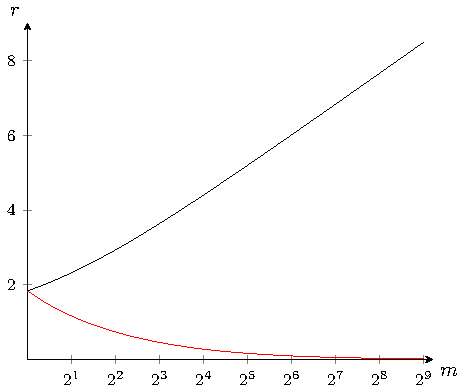
\includegraphics{overhead.pdf}%
    \caption{Bit da Aggiungere per Correggere un Errore Singolo}
\end{figure}

\subsubsection{Caching}

Si è discusso precedentemente di come l'accesso alla memoria centrale rallenti le operazioni svolte dal processore. Memorie veloci sono disponibili, ma solo per piccole dimensioni, non rappresentano quindi la 
soluzione a questo problema. Per cui per risolvere questo problema si inserisce una piccola memoria all'interno della CPU stessa, di dimensione molto minore della memoria centrale, in grado di memorizzare i dati 
necessari allo svolgimento delle istruzioni, velocizzando di gran lunga le istruzioni, poiché questa memoria interna ha la stessa velocità del processore. 
Questa zona di memoria interna si chiama cache, e memorizza le ultime zone di memoria acceduta dalla CPU, per evitare accessi ripetuti in memoria centrale. Inoltre memorizza le zone di memoria attorno a queste, 
le più probabili ad essere richieste dalla CPU. 
Rispetta due principi di località:
\begin{itemize}
    \item Temporale: Poiché una stessa zona di memoria verrà acceduta più di una sola volta dalla CPU, come l'aggiornamento di una singola variabile;
    \item Spaziale: Se serve una certa locazione di memoria, probabilmente verranno richieste anche le locazioni intorno a questa, come per un array. 
\end{itemize}     
Per cui vengono trasferiti interi blocchi di memoria nella cache ad ogni singola lettura in memoria centrale. 

Si definisce il cache hit ratio, la percentuale di volte che una parola letta, viene ritrovata nella cache, su $k$ letture di seguito. Poiché dopo la prima lettura l'intera zona di memoria viene salvata nella cache, 
si hanno $k-1$ cache hit, quando viene trovato nella cache, ed una singola cache miss, quando non viene trovato nella cache. Si ha quindi un cache hit ratio pari a:
\begin{equation}
    H=\displaystyle\frac{k-1}{k}
\end{equation}
Data questa metrica può essere quindi calcolato il tempo medio di accesso a memoria, dato il tempo di accesso alla memoria centrale $m$, ed il tempo di accesso alla cache $c$: 
\begin{equation}
    A=c+(1-H)\cdot m
\end{equation}
Per ogni cache miss, un intero blocco di memoria viene spostato nella cache. 

La cache è trasparente rispetto alla memoria centrale, ovvero il processore non è in grado di determinare se il dato che sta leggendo provenga dalla memoria centrale oppure dalla cache, l'unica differenza è la velocità 
di accesso. 

\subsubsection{Schede di Memoria}

Esistono diversi tipi di schede di memoria, ognuna con un certo numero di piedini, e di chip di memoria. Alcune presentano bit di parità, realizzati tramite un chip in più. 
Ogni tipologia di scheda di memoria è standardizzata, per permettere ai costruttori di realizzare schede di memoria in grado di comunicare correttamente con il processore. 
Le principali tipologie sono:
\begin{itemize}
    \item SIMM, ``Single Inline Memory Module'': memorie a 32 bit, utilizzano 72 piedini, e dalle 8 ai 16 chip di memoria di 128 MB ciascuno;
    \item DIMM, ``Double Inline Memory Module'': memorie a 64 bit, aventi tra i 120 e 240 piedini, con 8 chip di memoria da 256 MB;
    \item SO-DIMM, ``Small Outline-DIMM'': schede DIMM di dimensione ristretta utilizzate in notebook di piccole dimensioni;
    \item DDR/DDR2/DDR3/(M)DDR4/DDR5, ``Double Data Rate'': introducono un meccanismo di pipeline nella lettura e scrittura, e possono avere fino a 288 pin. 
\end{itemize}
Le memorie SIMM vengono utilizzate a coppie nei processori Pentium, per avere un bus dati a 64 bit. 
Ogni scheda di memoria DDR presenta una tacca diversa, per impedire che sia montata fisicamente su un supporto non valido. 

\subsubsection{Dischi Magnetici}

I dischi magnetici, o hard disk, termine usato per ogni memoria secondaria, sono memorie non volatili che si basano sulle proprietà elettro-magnetiche di alcuni materiali. 
Vengono realizzati tramite dei dischi di alluminio sovrapposti, di meno di dieci centimetri di diametro, con una densità di bit pari a 25 Gb/cm. I dati vengono memorizzati su traccie concentriche, divise in 
settori, ognuna di pochi micron in altezza, ogni settore contiene un migliaio di bit. Sono presenti circa 50000 tracce per centimetro del disco, larghe circa 200 nanometri. I bit vengono registrati verticalmente 
sulle tracce. Ogni settore presenta un preambolo per allineare la testina che legge i dati, i dati, ed un ECC ``Error-Correcting Code'', per correggere gli errori in lettura, poiché presenta una percentuale di 
errore relativamente elevata. Per cui la capacità formattata di un disco diminuisce del 15\% rispetto alla sua capacità effettiva. 
Questi dischi ruotano ad una velocità costante, tra i 5400 ai 10800 giri al minuto, o RPM, con una banda di 150 MB/s, leggendo un settore in pochi microsecondi: $t_A=3.5\,\mu\mathrm{s}$. 
Un braccio meccanico si sposta radialmente sul disco per leggere o scrivere i bit. Quando deve scrivere viene attraversato da una piccola corrente, generando un campo magnetico orientando in uno di due versi, per 
indicare uno zero oppure un uno,  le particelle magnetiche disposte sul disco. In lettura il disco non viene attraversato da corrente, ma quando la testina passa sopra ad un bit magnetico, questo genera un piccolo 
campo elettrico per induzione all'interno del braccio, misurabile come zero o uno in base al suo verso. 

Si utilizzano due misure di velocità del disco, il burst rate, la velocità da quando la testina è sopra il primo bit, ed il sustained rate, che calcola la velocità di trasferimento in un certo intervallo e comprende 
il tempo necessario per allineare la testina. Le traccie vengono sovrapposte a fino a formare un cilindro ed ogni lato di un disco può essere usato per memorizzare dati diversi. Ogni lato è quindi disposto di un suo 
braccio meccanico per leggere e scrivere i dati. 
Il tempo di accesso ad un dato può essere scomposto come il tempo di spostamento delle testine sul cilindro desiderato, ``Seek Time'', che dipende in parte dalla distanza attuale dalla testina, in una decina di millisecondi al massimo 
$t_S\approx5/10\,\mathrm{ms}$, ed il tempo di spostamento sul settore desiderato, ``Latency'', in un paio di millisecondi $t_L\approx3/6\,\mathrm{ms}$:
\begin{gather*}
    t_A=t_S+t_L
\end{gather*}

Ogni traccia concentrica presenta un numero diverso dei settori, poiché la velocità angolare dipende dalla distanza dal centro del disco, e bisogna mantenere la velocità di lettura di un singolo settore costante, 
altrimenti bisognerebbe modificare la velocità di rotazione del disco. Per gestire l'organizzazione dei dati sul disco sono necessarie delle capacità elaborative, sono quindi presenti dei processori 
specializzati nel disco, chiamati controllori di disco. 

Furono definiti degli standard per i dischi magnetici, il primo standard del IDE nato con il PC XT dell'IBM, aveva in totale 500 MB di memoria, ed una banda di pochi MB al secondo. 
Lo standard EIDE lo stende mediante lo schema LBA ``Logical Block Addressing'', un meccanismo di trasformazione da un indirizzo logico ad uno fisico, tramite una tabella di conversione, con una memoria massima 
gestibile di 128 GB. I dati vengono trasmessi tramite lo standard ATA ``AT Attachment'' e per le versioni successive ATAPI ``ATA PAcket Interface'', per ottenere una banda fino ai 100 MB/s. Da ATAPI-6 venne 
aumentata la massima memoria gestibile, fino ad un massimo di 128 PB, mentre da ATAPI-8 e successivi, il trasferimento si basa sullo standard SATA ``Serial ATA'', utilizzando connettori da meno bit, e tensioni 
più basse con velocità di trasmissione di decine di MB al secondo. Si utilizza una trasmissione seriale dei dati per risolvere un problema fisico di comunicazione sul bus, i bit viaggiano a diverse velocità 
sul bus, poiché attraversano linee strutturalmente diverse, questo fenomeno viene chiamato bus skew. Questo impone quindi un limite superiore alla velocità di trasmissione di un dato, mentre la trasmissione 
sequenziale dei bit, ovvero in forma seriale, non presenta limiti, e potenzialmente non presenta limiti alla velocità di trasferimento dei dati. 
Ulteriori accorgimenti utilizzano controller ed interfacce più intelligenti, SCSI ``Small Computer System Interface'', tramite bus con connessioni daisy chain, nella versione moderna Serial Attached SCSI per avere velocità di trasferimento dei 
dati fino a 10 Gb al secondo. 

\subsubsection{Dischi RAID}

Utilizzando più di un disco magnetico è possibile aumentare la velocità di trasferimento dei dati. Questa soluzione si chiama RAID ``Redundant Array of Inexpensive Disks'', usa più dischi per implementare un 
meccanismo di parallelismo in acceso ai dati, e meccanismi di resistenza ai guasti. Questo sistema si contrappone ai SLED ``Single Large Expensive Disk''. 
Nel RAID il singolo dato viene diviso e memorizzato su più dischi, tramite un processo di ``Data Striping'', in modo che possa essere acceduto in parallelo su più dischi. 

Sono possibili diverse configurazioni, da RAID 0 a 5, cambiando il numero dei dischi e la distribuzione dei blocchi di dati di un file su di essi. Il RAID di livello 0 consiste nel utilizzare $n$ dischi 
per memorizzare un singolo dato, guadagnano un fattore $n$ sia in lettura che in scrittura. Ma peggiore la frequenza degli errori, MTBF ``Mean Time Between Failures'', e non sono presenti meccanismi di 
resistenza ai guasti, non c'è ridondanza. 
Il RAID di livello 1 consiste in un RAID 0 dove tutti i dischi sono duplicati, una tecnica di shadowing, avendo la possibilità di resistere a guasti multipli, inoltre offre la possibilità di bilanciare il carico. 
Il RAID di livello 2 introduce un sistema di correzione di errori introducendo un bit di parità e dividendo il singolo dato a livello di word o di byte, ed ogni porzione di byte, nibble, o bit vengono salvati sul disco. In questo modo si ha 
una resistenza a guasti semplici e guadagna un fattore in lettura e scrittura in base al numero di dischi utilizzati. Ma per ottenere ciò i dischi devono essere sincronizzati in rotazione. Questo sistema è più efficiente all'aumentare dei 
dischi, per diminuire la percentuale di bit ridondanti da inserire. 
Il RAID di livello 3 rappresenta una versione semplificata del RAID 2, consente una distribuzione a livello di bit, ed un overhead contenuto, permette di recuperare i dati persi in caso di guasto sapendo quale 
disco è rotto. 
I RAID di livello 2 e 3 permettono di effettuare una sola operazione su disco per volta, poiché ogni operazione coinvolge tutti i dischi.  
Nel RAID di livello 4 si effettua uno striping a livello di blocco, ed i drive non sono sincronizzati, la strip dell'ultimo disco contiene i bit di parità dell'insieme di bit omologhi di tutte le altre strip. Riesce 
quindi a resistere ai guasti come un RAID 3, ma l'ultimo disco rappresenta un collo di bottiglia, poiché è necessario per ogni operazione di lettura. Per cui nel RAID 5 viene distribuita la strip di parità su tutti i 
dischi per minimizzare l'accesso ad un singolo disco. 

\subsubsection{Dischi a Stato Solido}

I ``Dischi'' a Stato Solido, SSD, chiamati dischi per motivi storici, memorizzano dati in maniera non volatile, sfruttano il fenomeno dell'``Hot-Carrier Injection'' dei transistor. Questa è una proprietà 
negativa dei transistor, dove gli elettroni che transitano il transistor possono superare lo strato isolante e rimanere in maniera permanente sui suoi componenti. 
Vengono quindi realizzate celle di memoria flash, a stato solido, quindi senza necessità di un'alimentazione, formate da vari transistor. 
I transistor vengono coperti da due strati isolanti, uno sopra ``Control Gate'' CG, ed uno sotto ``Floating Gate'' FG, per catturare le cariche. Alimentando il CG, vengono catturate le cariche sul FG, anche in assenza 
di alimentazione, e si misura la presenza di cariche poiché aumenta la tensione di commutazione. Si effettua quindi un test di commutazione a basso voltaggio per rilevare la presenza di cariche, ed in caso 
assegnare uno zero o un uno. 
Poiché sono presenti componenti puramente elettriche, questo sistema è estremamente veloce rispetto a dei dischi magnetici, con velocità di trasferimento nell'ordine dei centinaia di MB al secondo. Ma presenta dei 
difetti rispetto a HDD, poiché la frequenza di fallimenti è molto più elevata, e sono possibili un massimo di 100000 scritture prima di dover sostituire il dispositivo. 
Inoltre è molto più costoso di un disco magnetico, con un costo per GB di qualche euro, invece di qualche centesimo. Si addice per la sua compattezza alle applicazioni mobile, ed ai flash drive. La capacità può 
essere aumentata ulteriormente utilizzando celle multi-livello, e si può diminuire la frequenza di errore tramite una distribuzione uniforme delle letture e scritture sulle celle dell'unità, per evitare che si 
verifichi un guasto su una cella molto prima di un altra. 

\subsection{Dispositivi I/O}

I dispositivi di input e output forniscono all'utente la capacità di comunicare con il controllore, e sono collegati, come tutte le altre componenti, ad un bus e sono controllati da specifici processori, che 
trasferiscono autonomamente i dati in memoria, secondo la convenzione DMA ``Direct Memory Access'', senza dover passare per il processore. Questi dispositivi possono comunicare alla CPU tramite le interruzioni, e 
poiché condividono lo stesso bus, gli accessi devono essere regolati. 

La base di un controllore è costituita dalla scheda madre, dove sono presenti i connettori per i vari componenti. La scheda madre contiene i bus su cui vengono trasferiti i dati tra le varie componenti, su di essa 
vengono montate il processore, le schede di memoria, e collegati i dispositivi di memoria secondaria e di I/O connessi a corrispondenti connettori. Il bus è costituito da una serie di piste sul circuito stampato, 
spesso sono presenti più di uno secondo diversi standard. 

\clearpage

\section{Circuiti Digitali e Memorie}

Un calcolatore è una macchina realizzata a livelli, dove una macchina virtuale trasforma le istruzioni in un linguaggio fornito ad una macchina virtuale di livello inferiore, fino ad trasformare le istruzioni 
nel linguaggio macchina, eseguibile dal processore. Si utilizzano molti livelli intermedi per analizzare meglio la distinzione tra la compilazione o l'interpretazione della macchina virtuale, con cui interagisce 
l'utente ed il programmatore, e la macchina reale, che esegue a livello fisico le istruzioni sull'hardware. 
Si considera quindi una stratificazione che divide questi due livelli per permettere un'implementazione progressiva e modulare, in modo che un linguaggio di programmazione usato ad un certo livello non dipenda 
dall'hardware e siano presenti diverse soluzioni allo stesso livello. In questo modo è possibile ottenere una trasparenza all'utente finale ed alle applicazione che rende possibile di implementare diversi linguaggi 
di programmazione sulla stessa piattaforma ed introdurre lo stesso linguaggio su più piattaforme diverse. 


Ogni livello richiede una diversa astrazione del calcolatore. Il più basso livello L0 rappresenta la logica digitale, la combinazione delle porte logiche che formano le componenti principali del calcolatore. Il 
livello successivo L1 utilizza queste componenti per realizzare le microarchitetture ed implementa a livello di hardware il data path, i registri, l'ALU, i bus di controllo. A questo livello si sceglie se si 
tratta di un'esecuzione diretta o di un'interpretazione tramite microprogrammazione. Al livello successivo L2 si ha un processore unico, che richiede input e fornisce output in linguaggio macchina, è possibile 
quindi definire un set di istruzioni del linguaggio macchina dello specifico processore. Al livello successivo 
ancora L3 si ha un'interpretazione parziale tramite un sistema operativo che permette di gestire e virtualizzare le risorse del calcolatore. Salendo al livello superiore L4 è possibile scrivere programmai in 
linguaggio assembly, che vengono tradotti dal sistema operativo in linguaggio macchina, essenzialmente in corrispondenza uno ad uno con esso. In questo modo è possibile realizzare compilatori, per salire al livello 
successivo L5, dove sono presenti linguaggi di programmazione tradotti dal compiler in linguaggio macchina. Il livello 2 è il livello più basso a cui un utente può programmare, ma normalmente si programma 
al livello 5. 


\subsection{Algebra Circuitale}

Un circuito digitale è un circuito elettronico molto semplice, in cui gli ingressi e le uscite assumono solo due livelli, sono binari. Dato un set di input $i_1\cdots i_n$ un circuito digitale produce un set di 
output $o_1\cdots o_m$:
\begin{gather*}
    \begin{cases}
        o_1=f_1(i_1,\cdots,i_n)\\
        \vdots\\
        o_m=f_m(i_1,\cdots,i_n)
    \end{cases}
\end{gather*}

Queste funzioni $f_j$ vengono chiamate funzioni logiche o booleane, sono tutte funzioni aventi come dominio e codominio l'insieme contenente i due valori 0 e 1:
\begin{gather*}
    f:\{0,1\}\to\{0,1\}
\end{gather*}
Per cui sono possibili un numero finito di combinazioni e quindi di funzioni booleane, dati $n$ input. Sono possibili $2^n$ combinazioni di valori in input, e quindi $2^{2^n}$ possibili combinazioni in output, e quindi 
funzioni booleane distinte. Inoltre è possibile descrivere in maniera esaustiva una singola funzione booleana, tramite una tabella della verità, esprimendo tutte le possibili combinazioni in input ed il loro 
risultato in output:
\begin{center}
    \begin{tabular}{|c|c|c|c||c|}
        \hline
        $i_1$ &$\cdots$&$i_{n-1}$&$i_n$&$f$\\
        \hline\hline
        0&$\cdots$&0&0&$o_1$\\
        \hline
        0&$\cdots$&0&1&$o_2$\\
        \hline
        $\vdots$&$\ddots$&$\vdots$&$\vdots$&$\vdots$\\
        \hline
        1&$\cdots$&1&1&$o_m$\\
        \hline
    \end{tabular}
\end{center}

Con 1 bit in ingresso, ed in uscita, si hanno solo 4 funzioni disponibili: 
\begin{center}
    \begin{tabular}{|c||c|c|c|c|}
        \hline
        $x_1$&SET0&Buffer&NOT&SET1\\
        \hline\hline
        0&0&0&1&1\\
        \hline
        1&0&1&0&1\\
        \hline
    \end{tabular}
\end{center}
Le funzioni SET0 e SET1 impostano il valore ad uno o zero, indipendentemente dagli ingressi, mentre la funzione identità, restituisce il valore che gli viene passato, viene anche chiamata Buffer, e non 
rappresenta propriamente un operatore poiché non applica alcuna trasformazione agli ingressi o alle uscite. La funzione unaria più importante è il 
NOT che restituisce il valore opposto del valore che gli viene passato. 
Con 2 bit sono possibili 16 funzioni booleane, le più importanti sono AND ed OR, ma esistono altre funzioni di interesse come NAND, NOR, XOR, XNOR:
\begin{center}
    \begin{tabular}{|c|c||c|c|c|c|c|c|}
        \hline
        $x_1$&$x_2$&AND&OR&NAND&NOR&XOR&XNOR\\
        \hline\hline
        0&0&0&0&1&1&0&1\\
        \hline
        0&1&0&1&1&0&1&0\\
        \hline
        1&0&0&1&1&0&1&0\\
        \hline
        1&1&1&1&0&0&0&1\\
        \hline
    \end{tabular}
\end{center}

Se $x$ e $y$ sono due variabili booleane, l'AND si rappresenta come un prodotto $x\cdot y$, l'OR come una somma $x+y$ ed il NOT come $\bar{x}$. Date queste tre sole funzioni è possibile rappresentare ogni altre 
funzione booleana. Per cui data una funzione booleana ad $n$ variabili si definisce la Forma Canonica la seguente espressione:
\begin{equation}
    f:=\sum_{j=1}^m\prod_{i=1}^nx_{ij}^*
\end{equation}
Dove $x_{ij}^*$ vale $x_i$ oppure $\bar{x}_i$ e viene chiamato mintermine. 

\subsection{Porte Logiche}

Le porte logiche sono circuiti elementari che realizzano gli operatori dell'algebra booleana. Qualsiasi funzione booleana può essere realizzata dalle sole porte AND, OR e NOT. Inoltre può essere dimostrato come queste 
due porte possono essere rappresentate solamente usando le porte NAND o NOR, per cui queste due porte sono, singolarmente, complete e possono essere realizzate per realizzare qualsiasi circuito. 

Le porte logiche vengono rappresentate tramite i seguenti simboli circuitali:
\begin{figure}[H]%
    \centering
    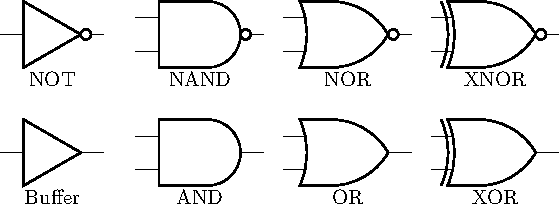
\includegraphics{porte-logiche.pdf}%
    \caption{Porte Logiche}%
\end{figure}
Il NOT si rappresenta sinteticamente come un pallino, quando si vuole negare l'entrata di una porta, o l'uscita per rappresenta le corrispettive porte negate. 
Le porte internamente sono realizzate da due transistor, tutte le porte a due input, e da un transistor, la porta NOT, tranne la porta Buffer poiché non modificando l'input non necessita di alcun componente circuitale 
aggiuntivo. I transistor permettono un tempo di commutazione ad altissima velocità. I valori di zero ed uno vengono rappresentati come valori alti o bassi di tensione, differenziati da pochi volt. 
%% TODO img. interne porte logiche (transistor), copia da E&E 


Di seguito si elencano le proprietà dell'algebra booleana:
\begin{center}
    \begin{tabular}{|c||c|c|}
        \hline
        Commutativa & $a+b=b+a$&$a\cdot b=b\cdot a$\\
        \hline
        Associativa & $a+(b+c)=(a+b)+c$ &$a\cdot(b\cdot c)=(a\cdot b)\cdot c$\\
        \hline
        Assorbimento & $a+(a\cdot b)=a$ & $a\cdot(a+b)=a$\\
        \hline
        Distributiva &$a\cdot(b+c)=(a\cdot b)+(a\cdot c)$& $ a+(b\cdot c)=(a+ b)\cdot(b+ c)$\\
        \hline
        Idempotenza & $a+a=a$ & $a\cdot a=a$\\
        \hline
        Esistenza di Minimo e Massimo & $a+1=1$ &$a\cdot0=0$\\
        \hline
        Esistenza del Complemento &$ a+\bar{a}=1$&$a\cdot \bar{a}=0 $\\
        \hline
        Esistenza di Elementi Neutri&$a+0=a$&$a\cdot1=a$\\
        \hline
        Legge di De Morgan &$\overline{a+b}=\bar{a}\cdot\bar{b}$ &$ \overline{a\cdot b}=\bar{a}+\bar{b}$\\
        \hline
        Assorbimento del Complemento &$a+\bar{a}\cdot b=a+b$ & $\bar{a}\cdot(a+\bar{b})=\bar{a}\cdot\bar{b}$\\
        \hline
    \end{tabular}
\end{center}
Si possono utilizzare queste proprietà per ottimizzare la realizzazione di circuiti logici, per diminuire il numero di transistor necessari. Permettono di semplificare la funzione booleana, oppure per utilizzare 
solo alcune porte per la scarsità di un certo tipo di porte sul mercato, come le porte AND. 

Si mostra ora la completezza delle porte NAND e NOR:
\begin{figure}[H]%
    \centering%
    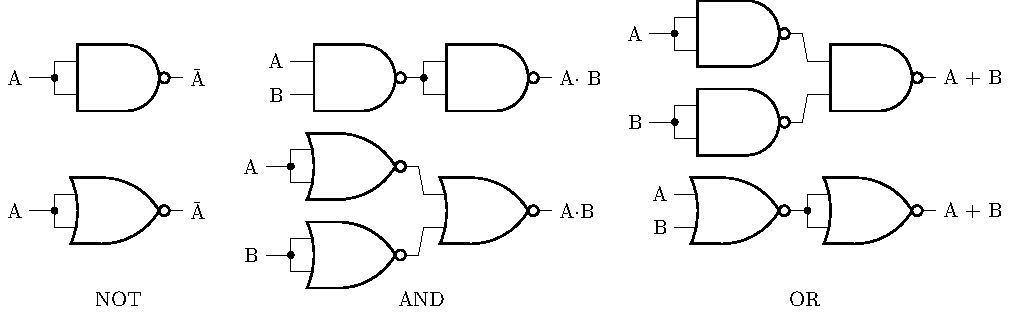
\includegraphics[scale=0.8]{completezza-nand-nor.pdf}%
    \caption{Completezza Porte NAND e NOR}%
\end{figure}

%% TODO porta xor tramite nand oppure and e or

Le porte logiche vengono vendute in circuiti integrati contenenti più di una porta, e connessi da piedini numerati all'esterno. Insieme al singolo chip vengono forniti le loro specifiche sulla posizione degli ingressi 
e le uscite delle varie porte contenute nel circuito. Devono essere sempre presenti gli ingressi di alimentazione VCC e di massa GND. Per orientare il circuito è presente una tacca o notch da una parte del chip, 
confrontandola con la scheda tecnica fornita. 
Questi chip vengono divisi in base al livello di integrazione:
\begin{itemize}
    \item SSI, ``Small Scale'': con al massimo una decina di porte;
    \item MSI, ``Medium Scale'': fino ad un centinaio di porte;
    \item LSI, ``Large Scale'': fino a $10^5$ porte;
    \item VLSI, ``Very Large Scale'': più di $10^5$ porte. 
\end{itemize}
Per questi chip i tempi di commutazione variano da $0.1$ a $10$ nanosecondi. 
Un processore è un VLSI, con molte porte e molti piedini, per fare spazio al numero di piedini necessari esistono diverse configurazioni la ``Dual Inline Packages'' DIPs, per circuiti di piccole dimensione 
presentano i piedini al lato, i ``Pin Grid Arrays'' PGAs, che presenta piedini su un'intera faccia del chip, ed i ``Land Grid Arrays'' LGAs, utilizzati per i processori moderni, come i PGAs presentano una matrice 
più fitta di piedini. 

I circuiti digitali possono essere divisi in due classi di circuiti, i combinatori ed i sequenziali. I primi combinano più input, e l'output dipende solamente dagli input, mentre nei secondi l'output dipende 
anche dallo stato del circuito. I circuiti combinatori vengono usati per realizzare i componenti di un processore, mentre i circuiti sequenziali per realizzare le componenti delle schede di memoria. 

\subsection{Circuiti Combinatori}

I circuiti combinatori sono circuiti digitali dove l'uscita dipende solamente dagli ingressi. 

\subsubsection{Multiplexer}

Un multiplexer è un circuito combinatorio avente $n$ ingressi di controllo, $2^n$ ingressi controllati, ed unica linea di output. Gli $n$ ingressi di controllo sono necessari ad identificare quale degli $2^n$ 
ingressi controllati da mandare in uscita. Internamente viene formato da $2^n$ porte AND per ogni ingresso controllato, ognuna collegata ad un ingresso di controllo ed ad un univoca combinazione degli 
ingressi di controllo. Tutte queste porte AND vengono poi collegate ad una singola porta OR, per permettere a qualsiasi ingresso sia stato abilitato di uscire. 

%% TODO img. multiplexer 2x4

Queste porte AND vengono chiamate porte di abilitazione, poiché effettivamente abilitano una uscita di un segnale. Vengono usati nella conversione parallelo-seriale di un bus, avente tante linee, ad un bus, avente 
una linea singola. Vengono abilitate tutte le linea, iterando su ogni linea, una alla volta, per convertire il segnale in seriale. Un multiplexer è in grado inoltre di implementare una qualsiasi funzione 
booleana di $n$ variabili. Le entrate di controllo rappresentano i mintermini, inoltre le entrate controllate vengono cablate a zero o ad uno a seconda che il mintermine compaia o meno nella forma canonica. 

\subsubsection{Decodificatore}

Un decodificatore è un circuito combinatorio a $n$ ingressi e $2^n$ uscite, dove una sola delle uscite assume valore uno, in base alla combinazione di valori di ingresso. Vengono usati per indirizzare una 
locazione di memoria, trasformando una sequenza di bit, nella corrispondente linea che identifica l'indirizzo. Effettua l'operazione inverse del multiplexer, trasformando una serie di dati seriali in parallelo. 

%% TODO img. decodificatore 2x4

\subsubsection{Comparatore}

Un comparatore è un circuito combinatorio che controlla se due stringhe in entrata sono identiche, comparando i bit omologhi delle due per valore, tramite tante porte XOR quanti sono i bit delle stringhe. Se tutti 
i bit sono uguali, allora ogni porta XOR restituisce 0, e quindi la porta NOR finale restituisce 1, altrimenti se restituisce 0, le due stringhe differiscono per almeno un bit. 

%% TODO img. comparatore 4x4

\subsubsection{Shifter}

Lo shifter è un circuito combinatorio in grado di traslare una data sequenza di bit in ingresso di un bit verso destra o sinistra, in base al valore del segnale di controllo C. 

%% TODO img. shifter 8

\subsubsection{Semi-Addizionatore}

Un semi-addizionatore o ``Half-Adder'' è un circuito combinatorio a due uscite e due ingressi, è in grado di sommare due bit tra di loro, restituisce il valore della loro somma, ed un eventuale riporto, o carry. Questo deve 
essere propagato se vengono sommate due stringhe di bit. Per effettuare questo tipo di somma si considera un ``Full-Adder''

%% TODO img. half-adder

\subsubsection{Addizionatore}

L'addizionatore è un circuito combinatorio a tre ingressi e due uscite, viene usato per effettuare la soma di numerali a più bit, poiché possiede un ingresso in più per inserire il riporto dell'addizione 
precedente. Per realizzare queste somme vengono collegati più Full-Adder uno dopo l'altro per effettuare la somma tra tutti i bit dei due numerali. In caso i numerali siano formati da molti bit, il tempo 
necessario alla propagazione del riporto è lineare con il numero di Full-Adder presenti nella catena, per cui nei processori vengono inseriti dei componenti in grado di calcolare solamente il riporto a priori, per 
poter effettuare la somma di tutti i bit in parallelo ed ottenere una complessità costante, invece che una complessità lineare per l'operazione. 

%% TODO img. full-adder



\end{document}